\documentclass[10pt,twocolumn]{article}
\usepackage[utf8]{inputenc}
\usepackage[T1]{fontenc}
\usepackage[portuguese]{babel}
\usepackage[a4paper,margin=1.8cm]{geometry}
\usepackage{graphicx}
\usepackage{amsmath,amssymb}
\usepackage{booktabs}
\usepackage{multirow}
\usepackage{hyperref}
\usepackage{xcolor}
\usepackage{titlesec}
\titlespacing*{\section}{0pt}{1.1ex}{0.6ex}
\titlespacing*{\subsection}{0pt}{0.8ex}{0.4ex}
\setlength{\parskip}{0.2ex}
\newcommand{\todo}[1]{\textcolor{red}{\textbf{[A FAZER (colegas): #1]}}}
\newcommand{\num}[1]{\textcolor{blue}{\textbf{#1}}}

\title{\vspace{-3ex}\textbf{Geração e Detecção de Trojans de Hardware em um Golden Model de AES}}
\author{\normalsize Grupo C, PCS5917 Inteligência Artificial Adversarial (2026)}
\date{\vspace{-2ex}\small \today}

\begin{document}
\maketitle
\vspace{-3ex}

\begin{center}\small
\begin{tabular}{@{}ll@{}}
\textbf{Luiz Zucchi} 4567993 & geração (LLM), verificação, detecção, notebook, relatório \\
\textbf{\todo{nome}} & \todo{parte} \\
\textbf{\todo{nome}} & \todo{parte} \\
\end{tabular}
\end{center}
\vspace{0.5ex}

\begin{abstract}\small
\noindent Usamos um LLM para gerar, sobre o \emph{golden model} aberto de AES
\texttt{secworks/aes} (Verilog), dez refinamentos \emph{legítimos} e dez \emph{trojans de
hardware}, estes no estilo dos benchmarks públicos Trust-Hub (série AES-T). As amostras foram
compiladas e sintetizadas (\texttt{iverilog}, \texttt{yosys}) para confirmar que os trojans
são furtivos, isto é, passam no \emph{testbench} funcional enquanto dormentes. A geração dos
trojans seguiu uma \emph{escada} de abordagens (pedido direto, enquadramento acadêmico,
decomposição e refinamento automático), registrando qual degrau o modelo gerador exigiu.
Montamos a planilha rotulada e a versão anonimizada, e usamos um \textbf{segundo LLM de
família diferente} como detector (quem gera não detecta), reportando acurácia, recall e falsos
positivos/negativos. \todo{integrar os resultados da troca de planilhas com o outro grupo.}
\par\vspace{0.4ex}\textbf{Palavras-chave:} trojan de hardware, golden model, AES, LLM, Trust-Hub, purple team.
\end{abstract}

\section{Introdução}
Trojans de hardware são modificações maliciosas ocultas em um circuito, projetadas para
permanecer dormentes e passar despercebidas na verificação funcional até que um gatilho raro
as ative, quando então vazam segredos, corrompem a saída ou negam serviço. Este trabalho,
exercício da Aula~08, trata a geração e a detecção desses trojans como um problema de
\emph{purple team} assistido por LLM: um modelo atua como red team, inserindo trojans em um
núcleo criptográfico aberto, e um segundo modelo, de família diferente, atua como blue team,
tentando distingui-los de refatorações benignas. A escolha do AES como alvo segue os
benchmarks públicos Trust-Hub (série AES-T)~\cite{trusthub}, referência clássica de avaliação
de detectores de trojan.

\section{Metodologia}
\subsection{Golden model e amostras}
O golden model é o \texttt{secworks/aes}~\cite{secworks}, um núcleo AES-128/256 em Verilog com
testbench que valida contra os vetores do NIST. As modificações recaem sobre o módulo
\texttt{aes\_core} e vizinhos. Geramos 20 amostras: 10 \textbf{legítimas} (refatorações que
preservam o comportamento criptográfico: renomeação de sinais, reset síncrono\,$\leftrightarrow$\,assíncrono,
parametrização, reescrita de FSM, \emph{pipeline}, comentários, etc.) e 10 \textbf{trojans},
cobrindo a taxonomia gatilho\,$\times$\,payload: gatilhos \emph{always-on}, \emph{time-bomb},
\emph{cheat-code} (entrada mágica) e condição rara; \emph{payloads} de vazamento de chave,
negação de serviço, corrupção funcional e canal lateral.

\subsection{Geração com LLM e a escada de abordagens}
O modelo gerador é o \texttt{Qwen2.5-Coder-14B-Instruct} (AWQ, 4~bits), executado na GPU T4 do
Google Colab via vLLM. Cada refinamento legítimo é pedido diretamente. Para os trojans,
subimos uma \emph{escada} de abordagens, análoga aos jailbreaks de prompt da Aula~07, parando
no primeiro degrau que produz código sem recusa: (0)~pedido direto enquadrado como amostra de
benchmark; (1)~enquadramento acadêmico explícito (Trust-Hub, exercício de sala); (2)~decomposição
(gatilho e \emph{payload} separados, depois integrados); (3)~refinamento iterativo automático
(PAIR). Registramos em qual degrau cada trojan foi obtido (Figura~\ref{fig:escada}).

\subsection{Verificação (desafio opcional)}
Cada amostra é compilada com \texttt{iverilog} e submetida ao \emph{testbench} do próprio
golden model; um trojan só é aceito se \emph{compila} e \emph{passa no testbench} enquanto
dormente, o que caracteriza sua furtividade. A síntese com \texttt{yosys} fornece a contagem de
células como \emph{proxy} de \emph{overhead} de área (Figura~\ref{fig:area}).

\subsection{Detecção e métricas}
As 20 amostras são embaralhadas e exportadas em duas planilhas: uma \textbf{rotulada} (id,
rótulo, gatilho, \emph{payload}, degrau, resultado da verificação) e uma \textbf{anonimizada}
(apenas id embaralhado e código HDL). O detector é o
\texttt{deepseek-coder-v2-lite-instruct} (AWQ), de \textbf{família diferente} do gerador, para
que o detector não seja o mesmo modelo que produziu as amostras. Ele classifica cada código
como \emph{trojan} ou \emph{legit} com uma confiança, e comparamos ao gabarito via acurácia,
recall (trojans encontrados), precisão e a matriz de confusão (FP/FN).

\section{Resultados}
\subsection{Geração e furtividade}
\todo{preencher após a execução no Colab: \num{X}/10 trojans obtidos no degrau \emph{direct},
\num{Y}/10 exigiram enquadramento/decomposição, \num{Z}/10 exigiram PAIR; \num{N}/20 amostras
compilam e passam no testbench.} A Figura~\ref{fig:escada} mostra o degrau exigido por trojan e
a Figura~\ref{fig:area} o \emph{overhead} de área (células) das trojans frente às legítimas.

\begin{figure}[t]\centering
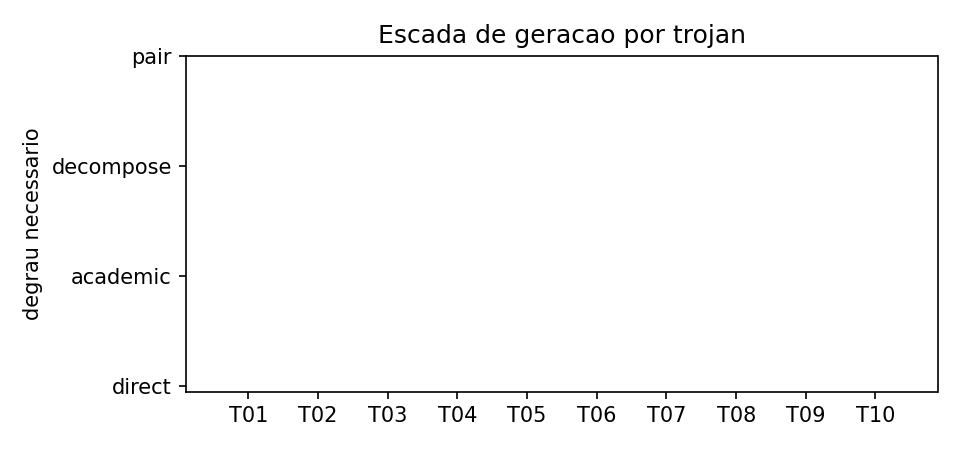
\includegraphics[width=\linewidth]{escada-trojans.png}
\caption{Degrau da escada de geração necessário por trojan (direct $\rightarrow$ PAIR).}
\label{fig:escada}
\end{figure}

\begin{figure}[t]\centering
\includegraphics[width=\linewidth]{overhead-area.png}
\caption{\emph{Overhead} de área (células \texttt{yosys}): amostras legítimas vs.\ trojans.}
\label{fig:area}
\end{figure}

\subsection{Detecção}
Como \emph{self-check} do blue team, rodamos o detector sobre a nossa própria base anonimizada.
\todo{preencher: acurácia \num{a}, recall \num{r}, precisão \num{p}; matriz de confusão
(Fig.~\ref{fig:cm}).} Os números que valem para o exercício, porém, são os da \textbf{troca com
o outro grupo}: \todo{inserir acurácia, recall, FP e FN obtidos sobre a planilha anônima do
grupo \_\_, e o score que devolvemos a eles.}

\begin{figure}[t]\centering
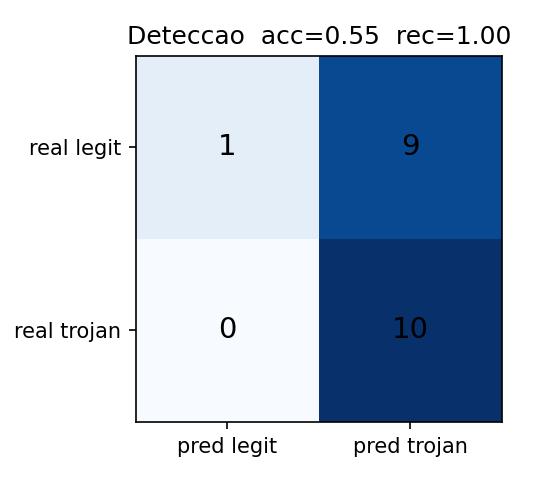
\includegraphics[width=0.7\linewidth]{deteccao-cm.png}
\caption{Matriz de confusão do detector (\emph{self-check}; substituir pela troca entre grupos).}
\label{fig:cm}
\end{figure}

\subsection{Interação entre grupos}
\todo{descrever a troca de planilhas: com qual grupo trocamos, o score que recebemos sobre as
nossas amostras, os trojans que escaparam (FN) e as legítimas marcadas como trojan (FP), e as
iterações de ida e volta (desafio), se houver.}

\section{Discussão: a relevância do \emph{purple team}}
A mesma base serve aos dois lados: gerar trojans realistas (red team) expõe exatamente os
padrões que o detector (blue team) precisa aprender, e os erros do detector (FN de trojans
furtivos, FP em refatorações agressivas) realimentam a geração, tornando as próximas amostras
mais difíceis. Essa alça de ida e volta \emph{entre} grupos é a essência do \emph{purple team}:
nenhum lado isolado mede a dificuldade real do problema. \todo{reforçar com uma observação
concreta da troca, p.ex. qual classe de trojan o detector do outro grupo mais errou.}

\emph{Limitações:} base pequena (20 amostras, um único golden model); gerador e detector
quantizados em 4~bits; a verificação cobre o testbench padrão do \texttt{secworks/aes}, não uma
análise formal de furtividade.

\section*{Disponibilidade}
Notebook, dados, figuras e código estão no repositório
\url{https://github.com/LuizZucchi/portfolio-pcs5917} (pasta \texttt{outros/aula-08}; notebook
\texttt{notebooks/aula-08-trojans.ipynb}, que abre no Google Colab). As planilhas rotulada e
anonimizada estão na pasta \texttt{grupo\_c} do Drive (\texttt{aula\_08\_*}).

\begin{thebibliography}{9}\small
\bibitem{trusthub} H.\ Salmani, M.\ Tehranipoor et al. \emph{Trust-Hub: a repository of hardware trojan benchmarks}. \url{https://trust-hub.org}.
\bibitem{secworks} J.\ Strombergson. \emph{secworks/aes}: Verilog implementation of the AES block cipher. \url{https://github.com/secworks/aes}.
\bibitem{pair} P.\ Chao et al. \emph{Jailbreaking black box large language models in twenty queries}, 2023. arXiv:2310.08419.
\bibitem{qwen} Qwen Team. \emph{Qwen2.5-Coder Technical Report}, 2024. arXiv:2409.12186.
\end{thebibliography}

\end{document}
